% HMSS 2026 / IEEE conference paper
% HMSS 2026 uses the A4 IEEE Manuscript Template for Conference Proceedings.
% Build: PATH="/Library/TeX/texbin:$PATH" latexmk -pdf main.tex

\documentclass[conference,a4paper]{IEEEtran}

% Uncomment only if you need a funding footnote in the first-page author block.
% \IEEEoverridecommandlockouts

\usepackage{cite}
\usepackage{amsmath,amssymb,amsfonts}
\usepackage{graphicx}
\usepackage{booktabs}
\usepackage{url}
\usepackage[hidelinks]{hyperref}

\begin{document}

\title{CWC Health: Co-Designing a Privacy-Preserving Mobile Health Navigation Platform for Community Wellness Centers}

\author{
\IEEEauthorblockN{Carolyn E. Sartor\IEEEauthorrefmark{1},
Margaret Swarbrick\IEEEauthorrefmark{2}\IEEEauthorrefmark{3},
and Amy B. Spagnolo\IEEEauthorrefmark{2}\\
Karim Smires\IEEEauthorrefmark{4}, Kareem Kholaif\IEEEauthorrefmark{4},
and Sasan Haghani\IEEEauthorrefmark{4}}
\IEEEauthorblockA{\IEEEauthorrefmark{1}Department of Psychiatry, Rutgers Robert Wood Johnson Medical School\\
\IEEEauthorrefmark{1}Center for Population Behavioral Health\\
\IEEEauthorrefmark{1}Rutgers Institute for Health, Health Care Policy, and Aging Research\\
\IEEEauthorrefmark{1}112 Paterson Street, New Brunswick, NJ 08901-1293, USA\\
\IEEEauthorrefmark{2}Rutgers ScarletWell\\
\IEEEauthorrefmark{3}Graduate School of Applied and Professional Psychology\\
\IEEEauthorrefmark{3}Center of Alcohol and Substance Use Studies\\
\IEEEauthorrefmark{4}Department of Electrical and Computer Engineering\\
\IEEEauthorrefmark{4}Rutgers University\\
Piscataway, NJ 08854, USA}
}

\maketitle

\begin{abstract}
This paper reports the initial design of CWC Health, a privacy-preserving mobile
health navigation platform for Community Wellness Centers (CWCs). The intended
users are adults who may experience poverty together with mental health,
substance-use, or co-occurring physical health challenges. The design was
informed by CWC members and peer support specialists through eight focus groups
and Qualtrics pre-surveys, with input from clinicians and a community advisory
board. Findings emphasized trusted local resources, plain language, support from
peers, and explicit limits on data collection. The resulting design uses four
tabs---\emph{Nearby}, \emph{My Health}, \emph{Learn}, and \emph{More}---and a
persistent \emph{Help Now} control. \emph{Nearby} supports town-based resource
discovery and optional one-shot location use. \emph{My Health} stores
user-entered information on the device behind optional access controls.
\emph{Learn} provides plain-language wellness information, \emph{More} provides
app and peer-support guidance, and \emph{Help Now} provides urgent contacts. The
platform requires no user account and includes no third-party analytics. It examines
how much contextually personalized health support a mobile app can provide while
retaining as little sensitive user data as possible. Clinical efficacy and
usability outcomes are outside the scope of this paper.
\end{abstract}

\begin{IEEEkeywords}
mobile health, health navigation, privacy by design, data minimization,
co-design, community wellness, digital health
\end{IEEEkeywords}

\section{Introduction}
People seek health information through search engines, health websites, social
media, providers, and personal networks. Finding information does not ensure that
it is credible or usable. Reviews report difficulty evaluating online health
information across age groups and sources
\cite{Jia2021OHIS,DiazHernandez2024HealthInfo,Zhao2022OlderOHIS}, while a US
survey found widespread exposure to health content on social media together with
concern that much of it is misleading~\cite{Pedroso2026SocialMedia}. Social
prescribing similarly recognizes that health support includes connections to
non-medical community resources~\cite{Lancet2025SocialPrescribing}. CWC Health
does not attempt to replace these sources or assemble a clinical care pathway.
It provides one place to reach local resources, basic health information, and
urgent contacts.

Mobile health (mHealth) tools can extend access, but access alone does not produce
sustained use. A systematic review identified technology, language, usability,
trust, and interpersonal support as recurring barriers for culturally and
linguistically diverse groups~\cite{Whitehead2023Barriers}. Work in youth
services and serious mental illness adds privacy, sustainability, and digital
literacy concerns~\cite{Ding2025mHealth,Dwyer2025TechUse}. These barriers are
especially relevant for people with limited income, unstable access to devices,
or prior reasons to distrust digital systems. What is missing is not another
feature-heavy health app, but a tool people can understand and trust without
providing extensive personal information.

Participatory health research offers a way to define that tool with, rather than
for, its intended users. Community-based participatory research emphasizes shared
decisions with community partners~\cite{Opara2025CBPR}; co-production work adds
context-specific design and lived-experience leadership
\cite{PapastavrouBrooks2023Principles,Epp2025CoLeadership}. Recent projects
co-designed clinical or recovery-oriented apps with lived experts, clinicians,
and advisory boards~\cite{Darcey2024A4iO,Deshais2026WECM}. CWC Health applies
the same principle to health navigation rather than clinical decision support.
Its focus on CWC members, peer support specialists, and a community advisory
board also responds to warnings that the participatory label can be used without
meaningful shared influence~\cite{Veldmeijer2025Participatory}.

IEEE health-app work has explored neural-network support for resource-poor
community settings and interactive self-management interfaces
\cite{Pasha2020CommunityHealth,Chiu2021SelfManagement}. CWC Health differs by
avoiding automated diagnosis and continuous monitoring. It centers
user-directed navigation, peer-supported use, and local-only storage. Privacy by
design treats these limits as defaults rather than later additions
\cite{Cavoukian2010PbDWorkshop}. Prior studies document privacy-policy gaps in
mHealth apps and concern when users learn how often apps access location
\cite{Alfawzan2022mHealthPrivacy,Almuhimedi2015LocationShared}. CWC Health
therefore asks: \emph{How much useful, contextually personalized health support
can a mobile application provide while collecting and retaining as little
sensitive user data as possible?} Here, personalization means context chosen by
the user, such as a town and health information stored on the phone. It does not
mean diagnosis or treatment recommendation.

This paper reports a needs assessment with CWC members and peer support
specialists, explains how the findings shaped the product, and presents the
resulting mobile design. Its contributions are (i) empirical evidence about
health-information needs, digital hesitancy, privacy concerns, and support
preferences in CWCs; (ii) an explicit mapping from those findings to the
interface; and (iii) a data-minimizing design for local resource discovery and
personal health organization without accounts, analytics, or retained location
history.

\section{Study Design and Aims}
This needs assessment examined how community feedback should inform a mobile
health-navigation app for CWCs operated with Collaborative Support Programs of
New Jersey (CSPNJ). The aims were to understand how members and peer support
specialists seek health information, what local resources they use, what makes a
health app usable or untrustworthy, and what support they want when using one. A
community advisory board with lived experience contributed to recruitment,
interpretation, and feature prioritization.

\subsection{Setting and Participants}
The Rutgers Human Research Protection Program approved the study as Exempt~3b
(IRB Pro2025002116; 19~November~2025). The study was determined to be minimal
risk. Consent covered recording, confidentiality, and the right to withdraw.
Recruitment targeted English-speaking adults age 18 or older who could consent
and participate in app-related discussion. Participants were drawn from CSPNJ
CWCs across New Jersey regions.
Peer support specialists were recruited for virtual sessions so staff at multiple
sites could join without travel. Members were recruited for in-person sessions at
the centers where they already receive services. Eight moderated groups were
completed: two virtual peer-support groups in February 2026 and six in-person
member groups across three site days in March 2026. The member groups met in
Glassboro, Jersey City, and Plainfield.
Compensated attendance records show $n{=}7$ peer support specialists in virtual
groups and $n{=}38$ CWC members in person. Each participant received a \$50 gift
card.

\subsection{Procedures}
Virtual sessions used Zoom with a waiting room and host-only audio recording.
In-person sessions met in private rooms. Consent procedures were completed before
discussion and recording, and members completed a short Qualtrics pre-survey on
a laptop or phone. Facilitator scripts covered health information
access, local resources, technology and health apps, trust/distrust, and support
preferences. Session scripts allotted 75--90 minutes including consent and survey
administration. Recordings were
transcribed and de-identified before analysis.

\subsection{Pre-Survey}
Members and peer support specialists completed Qualtrics pre-surveys on
demographics, smartphone access and comfort, health information seeking, and
preferred help for using a health app. Response counts vary by item because
Qualtrics skip logic routed respondents without smartphone access past later
phone-specific questions. Member demographics are therefore reported for
$n{=}41$, smartphone-specific member items for $n{=}27$, and peer-support items
for $n{=}9$--10 depending on the question. Attendance and survey records were not
linked at the participant level.

\subsection{Analysis}
Focus-group transcripts were analyzed with iterative qualitative content
analysis. Reviewers familiarized themselves with each transcript and wrote
memos. A codebook combined deductive codes from the study aims/guide with
inductive codes from participant language. Two reviewers independently coded
meaning units, met to resolve disagreements, and used a third reviewer as
adjudicator when needed. Codes were grouped into higher-order categories for
member and peer-support summaries. Trustworthiness relied on multiple coders,
consensus meetings, memoing, and an audit trail of coding decisions.

\section{Needs-Assessment Findings}

\subsection{Pre-Survey Results}
Among members with demographic responses ($n{=}41$), 46\% were unemployed and
12\% were unemployed and receiving SSI/SSDI; 48\% reported some form of unhoused
status (24\% shelter, 24\% unsheltered). Highest completed education was often high school or less (44\% high school
or equivalent; 17\% some high school without a diploma). Just over half
(54\%) were age 45 or older. Smartphone access was incomplete: 63\% of members
reported a smartphone ($n{=}41$ base for that item), and most without a phone
also lacked regular access to someone else's device.

Among members routed to smartphone-specific items ($n{=}27$), use was frequent
(81\% multiple times a day), mostly Android (78\%), with mean comfort $3.41$ on
a 1--4 scale.
Health-app use was low: 63\% used health apps ``rarely'' or ``never.'' Most of
these respondents sought health information (89\%), often daily (46\%), mainly
via internet search (67\%), then providers (38\%) and friends/family (33\%).
Mean confidence finding health information was $3.26$ / 4. A large majority
(89\%) said a smartphone health app would be helpful, and 67\% wanted help using
one. Preferred help formats included video walkthroughs (42\%) and peer support
specialists (33\%). Members most often learned about wellness resources by word
of mouth (59\%) and family/friends (48\%).

Peer-support pre-survey items ($n{=}9$--10) showed high smartphone comfort
(mean $4$ / 4 where reported) and similar interest in a helpful health app, with
staff often positioned as the people who already help members navigate
technology.

\subsection{Member Focus-Group Themes}
Member discussions emphasized physical health routines (appointments,
medications, exercise, diet), mental health and recovery practices, and social
connection through CWCs and peers. Holistic, multi-domain wellness descriptions
were common. Information seeking mixed internet and AI tools with providers and
caseworkers, but experiential and peer knowledge were highly valued.
Action-oriented needs stood out: participants wanted next steps, clinics to
call, and practical guidance rather than abstract content alone. Resource access
centered on trusted local people and places, including CWCs. Barriers included
transportation, fragmented services, and low awareness of programs.

Digital tool hesitancy was frequent. Some members preferred phone appointments
over apps, disliked apps, or relied on a relative or caseworker to operate
technology. Plain language and walkthrough support were recurring requests.
Privacy and trust concerns covered scams, data misuse, and security; trust was
often placed in specific community staff or peers rather than generic platforms.

\subsection{Peer Support Specialist Themes}
Peer-support discussions (28 coded excerpts in the staff summary table) stressed
health information seeking, resource access, and ambivalence about digital tools:
convenience versus misinformation, and difficulty sustaining app use. Staff
wanted simple interfaces, reminders, credentialed content, and support for
self-tracking of medications and appointments. Technology support needs were
prominent from the staff vantage point (staff-assisted navigation and
institutional support). Structural barriers for members, including phone loss and
unstable housing, were described explicitly.

\section{Discussion}
The findings show a clear gap: many CWC members already use smartphones often, but
health apps are rare, trust is fragile, and help is expected from peers and
staff. ``Personalized'' support in this project means contextual access (a town
search, optional one-shot location, local listings, on-device health
organization), not diagnosis or treatment recommendation. Data minimization is a
design requirement here, not an add-on. Participants named scams,
surveillance-like collection, and login burden as reasons to avoid apps. These
concerns align with documented privacy-policy gaps in women's mHealth apps and
users' reactions to unexpected location
access~\cite{Alfawzan2022mHealthPrivacy,Almuhimedi2015LocationShared}.

The product is intentionally narrow. It navigates to care and education but does
not replace peer support, clinical portals, or crisis counselors. Gould et al.
evaluate caller outcomes after Lifeline calls~\cite{Gould2025Lifeline988}; CWC
Health's one-tap 988 entry is a navigation affordance, not a clinical crisis
service. Co-design with members and peer
specialists, plus a community advisory board, is how the team tries to avoid
``participatory'' labeling without shared decision-making
\cite{Veldmeijer2025Participatory,Epp2025CoLeadership}.

The design implications are summarized in Table~\ref{tab:theme_map}. Requests
for action-oriented local information motivated \emph{Nearby}. Distrust of
data-heavy apps and login burden motivated the no-account, no-analytics approach
and optional rather than continuous location use. Plain-language requests
motivated short, source-labeled material in \emph{Learn}. Appointment and
medication self-management needs motivated local storage in \emph{My Health}.
Peer-supported onboarding and urgent access motivated assistance in \emph{More}
and the persistent \emph{Help Now} control. These are design responses to the
needs assessment, not usability or clinical outcomes.

\begin{table}[!t]
\caption{Needs-assessment findings and product responses}
\label{tab:theme_map}
\centering
\begin{tabular}{@{}p{0.46\columnwidth}p{0.46\columnwidth}@{}}
\toprule
\textbf{Finding} & \textbf{Product response} \\
\midrule
Local resources and practical next steps & \emph{Nearby}; Call, Text, Directions \\
Distrust of data-heavy apps and logins & No accounts or analytics; optional location \\
Plain language and trusted sources & Source-labeled \emph{Learn} articles \\
Appointments and medication organization & Local-only \emph{My Health} records \\
Peer help and urgent access & \emph{More} assistance; persistent \emph{Help Now} \\
\bottomrule
\end{tabular}
\end{table}

\subsection{Limitations}
The focus-group and pre-survey samples are tied to participating CSPNJ sites and
English-speaking inclusion criteria. They are not a statewide probability
sample. Attendance and pre-survey records are separate, and item-level response
counts vary. The app has not yet undergone usability or clinical evaluation.
OSM coverage, hours, and contact fields also vary by resource and region
\cite{Haklay2010OSM,Mara2025OSMGoogleAmenities}. The team does not independently
verify every listing. No clinical outcomes are claimed.

\begin{figure*}[!t]
\centering
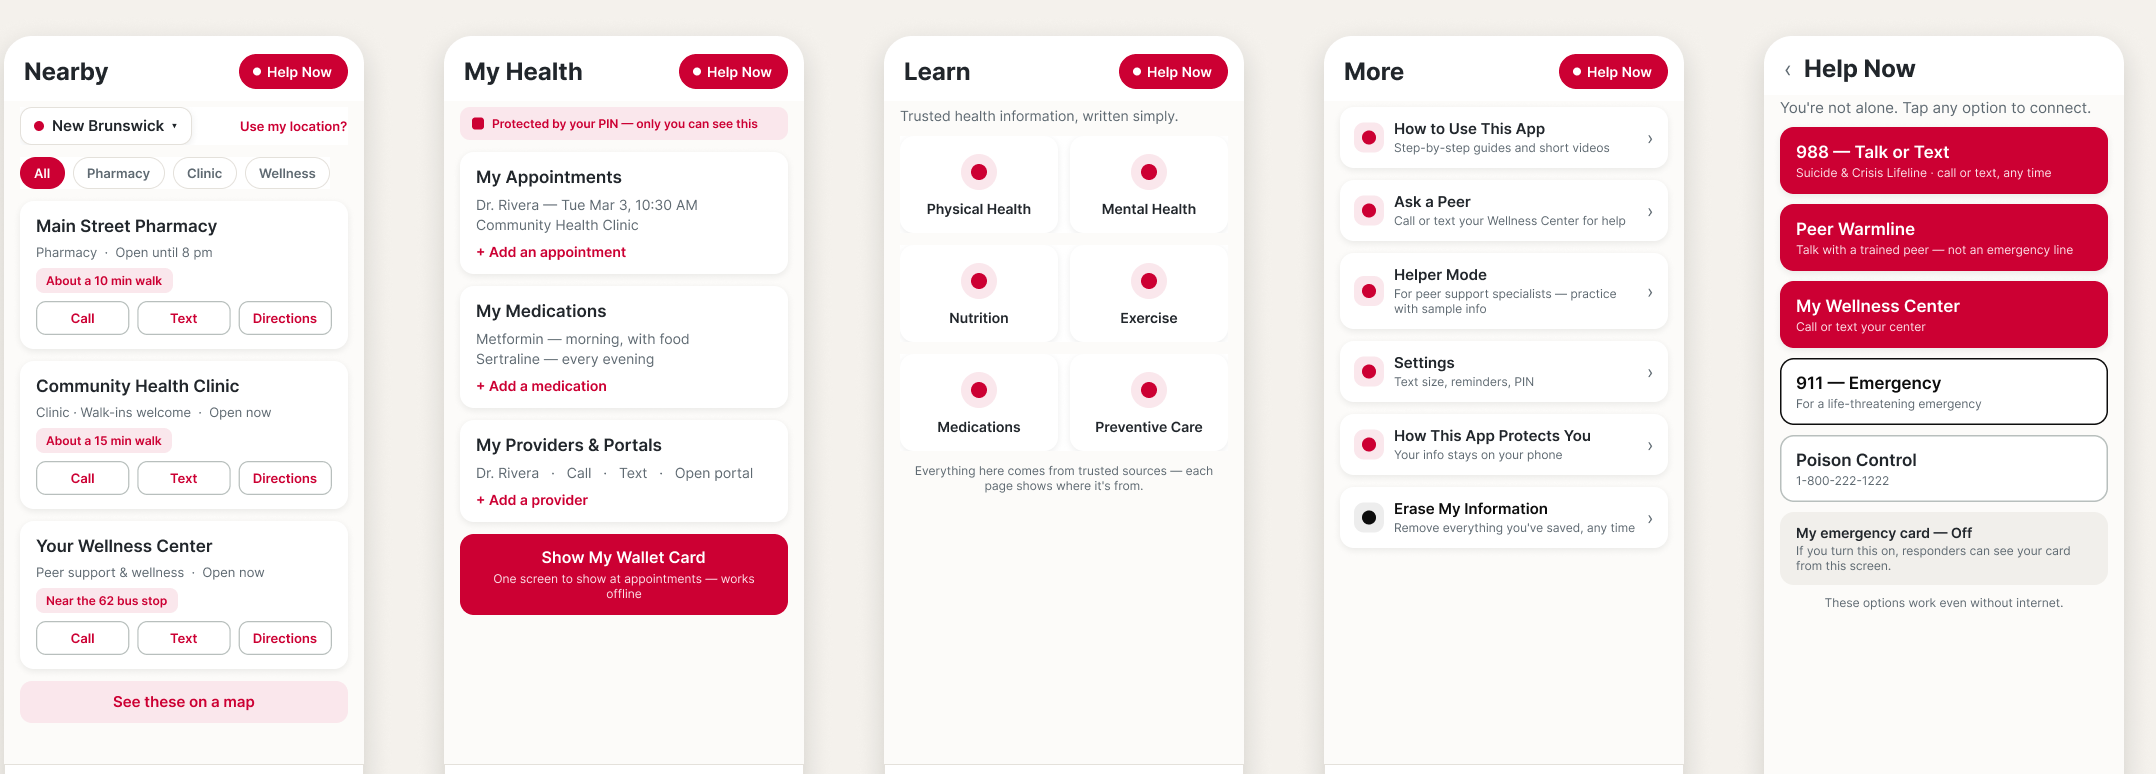
\includegraphics[width=\textwidth,height=0.32\textheight,keepaspectratio]{figures/ui_screens.png}
\par\vspace{-0.6ex}
\makebox[\textwidth][c]{\makebox[0.19\textwidth]{(a)}\makebox[0.19\textwidth]{(b)}%
\makebox[0.19\textwidth]{(c)}\makebox[0.19\textwidth]{(d)}\makebox[0.19\textwidth]{(e)}}
\caption{CWC Health interface. (a)~\emph{Nearby} lists local resources and
provides Call, Text, and Directions actions. (b)~\emph{My Health} organizes
user-entered appointments, medications, providers, and a wallet summary on the
device. (c)~\emph{Learn} presents plain-language material across the eight
dimensions of wellness. (d)~\emph{More} provides the walkthrough, peer
assistance, helper mode, settings, privacy information, and erase controls.
(e)~\emph{Help Now} provides persistent access to urgent and local contacts.}
\label{fig:ui}
\end{figure*}

\section{System Design}

\subsection{Design Goals and Application Structure}
CWC Health is a navigation system, not a clinical decision-support system. It
helps users find care, organize their own health information, read
source-labeled guidance, and reach urgent contacts. It does not diagnose or
recommend treatment. Three goals guide the design: collect as little data as
possible, present a layout members can navigate with peer support, and support
resource discovery without continuous location tracking.

The cross-platform Flutter client~\cite{FlutterDocs2026} has four bottom tabs
and a persistent header control (Fig.~\ref{fig:ui}). \emph{Nearby} finds
pharmacies, clinics, urgent care, and wellness resources and offers Call, Text,
and Directions actions. \emph{My Health} organizes user-entered appointments,
medications, providers, portal details, and a wallet summary on the device.
\emph{Learn} presents stable, plain-language material organized around the eight
dimensions of wellness. \emph{More} contains the walkthrough, peer assistance,
helper mode, accessibility settings, privacy information, training resources,
and data-erasure controls. The persistent \emph{Help Now} control reaches urgent
and local support numbers from any tab.

\subsection{Privacy and Data Minimization}
The design has no user accounts, stores no external login credentials, and
includes no third-party analytics SDKs. A selected town and the last successful
town listing may be cached on the device. Coordinates requested through
\emph{Use my location} remain in memory for that lookup and are not written to
storage. The app keeps no location history and performs no background location
tracking. \emph{My Health} uses an optional PIN, encrypted on-device records,
and a clear-data action. These controls implement privacy by design through
limits on collection and retention, not only through disclosure
\cite{Cavoukian2010PbDWorkshop}.

\subsection{Location-Aware Nearby Services}
The \emph{Nearby data path} is the sequence that turns a user-selected origin
into resource cards. It is \emph{town-first}: the primary path accepts a town
name, geocodes it through Nominatim~\cite{NominatimDocs}, and queries
OpenStreetMap (OSM) Overpass for nearby resources~\cite{OverpassDocs}. Location
permission is therefore not required. A user may instead choose \emph{Use my
location}, which supplies a one-shot coarse origin for that request. OSM and
commercial amenity sources differ in coverage, so the interface labels listings
as public map data that the team has not independently verified
\cite{Haklay2010OSM,Mara2025OSMGoogleAmenities}.

Figure~\ref{fig:nearby_pipeline} shows both origin choices and the failure path.
The client tries multiple Overpass mirrors because a community-center room may
share one rate-limited public IP address. Google Places is optional; a missing
key or failed request does not prevent the OSM lookup. Returned listings are
deduplicated and time-stamped. Successful town results are cached locally. When
all live sources fail, the app may show the last successful town result with its
original timestamp; if no cache exists, it shows an unavailable message and a
Try again action. It does not present bundled demonstration names as live data.
Missing or unparseable opening-hour fields are labeled ``Hours not listed.''

\begin{figure}[!t]
\centering
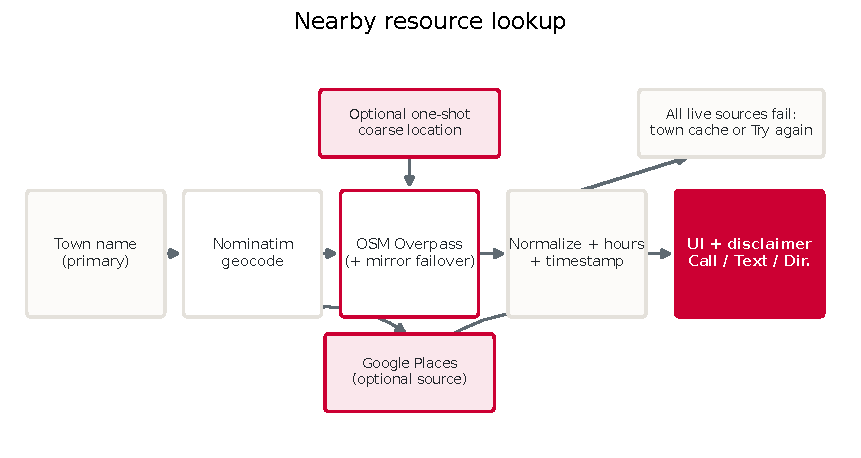
\includegraphics[width=\columnwidth]{figures/nearby_pipeline.pdf}
\caption{The \emph{Nearby} resource lookup. Town entry is the primary origin;
one-shot coarse location is optional. OSM is the supported live source, Google
Places is optional, and source failure leads to a timestamped cache or an
explicit retry state.}
\label{fig:nearby_pipeline}
\end{figure}

\subsection{Personal Information, Learning, and Help}
\emph{My Health} keeps appointments, medications, providers, portal references,
and a wallet card in an encrypted local store. Entries are optional and can be
erased. \emph{Learn} uses named sources and stable guidance rather than generated
answers or links that the team cannot maintain. \emph{More} includes helper mode,
which hides personal fields while a peer demonstrates the app. \emph{Help Now}
places 988, 911, Poison Control, peer helplines, and local contacts within two
taps. This is a navigation affordance, not a substitute for crisis care.
The contact numbers are stored on the device so the dialer can be opened without
an internet connection.

\section{Future Work}
The needs assessment produced a set of design requirements, and this paper
reports the interface derived from them. The next step is structured usability
testing with CWC members and peer support specialists. Planned sessions will use
guided tasks and think-aloud feedback to assess whether participants can find
local resources, enter and remove personal information, identify \emph{Help Now},
and understand the privacy model. The study will also examine text readability,
language clarity, trust in map and learning content, behavior across Android and
iOS devices, and the support that peer specialists need when assisting members.
Findings will guide interface refinement and the development of in-person and
virtual training materials. Participant counts and procedures will follow the
approved protocol in effect when testing begins.

\section*{Acknowledgment}
The authors thank the research assistants, community advisory board, CWC staff
and members, and peer support specialists who contributed to the needs assessment
and product design. This work was supported by a Rutgers Office of the Vice
Provost for Research pilot award.

\bibliographystyle{IEEEtran}
\bibliography{references}

\end{document}
